% Intro
This section describes the architectures of the legacy and new systems that will be run and measured in the experimental part of this thesis. The section is divided into four sections as each schema presented shows the protocol step by step.

\subsection{Legacy system - Writing}
\label{subsec:legacy_sys_writing}

Figure \ref{fig:featurestore_writing} shows the legacy Hopsworks Feature Store write process from the client on to the Offline Feature Store. The process is mainly split into two sychronous parts: upload and materialization. In the upload step the pandas data frame given as input is converted into rows and sent one row at a time to Kafka. Then, when the upload is finished the client is notified. Asynchronously, a Spark job keeps running in the cluster since the Hopsworks cluster was started, which is the Hudi Delta Streamer. This job periodically retrieves messages from Kafka, and then once it retrieves a full table it writes it in a column oriented format to Apache Hudi, that sits on top of a \gls{HopsFS} system. Once the materialization is completed the Python client is also notified of completion.

As in the pipeline, the upload and the materialization are two different parts of the process that do not act synchronously. During the experimental part of the thesis, to be able to measure the latency of the whole process without having to account for the Hudi Delta Streamer data retrieval period, the materialize function was called, which allows to perform the materialization on call instead of waiting the period. This enabled the experiments to retrieve accurate data on the total latency of the process.

\todo[inline]{Insert link to appendix for larger diagram}

\begin{figure}
    \begin{center}
      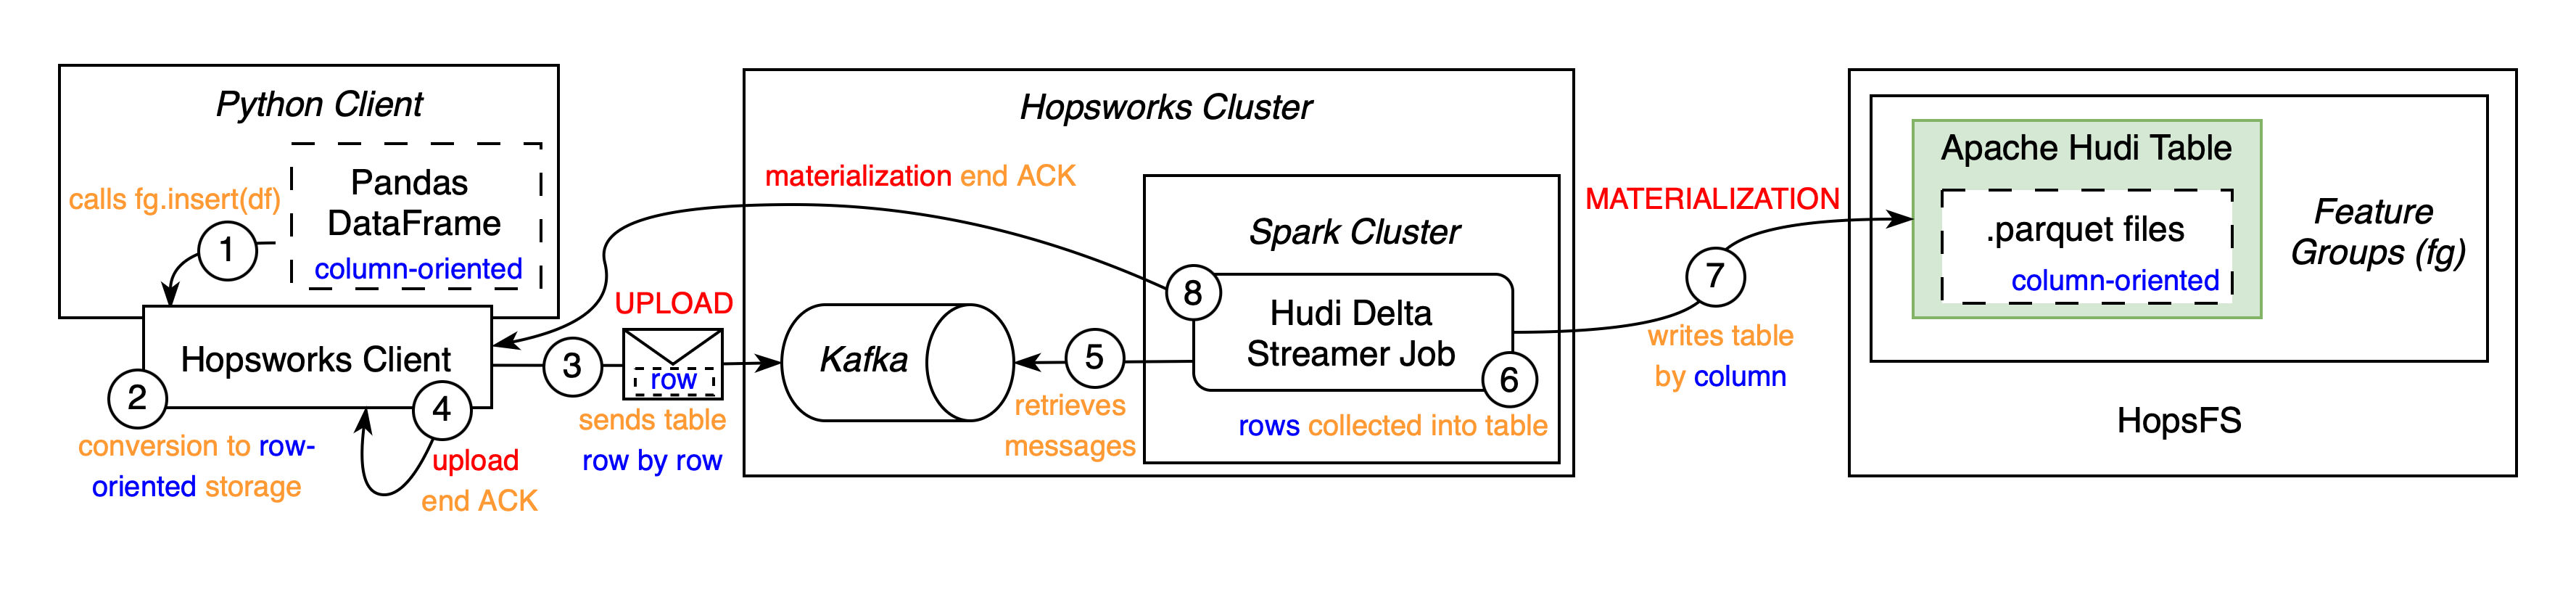
\includegraphics[width=\textwidth]{figures/2-background/FeatureStore-writing.png}
    \end{center}
    \caption{Legacy system writing process}
    \label{fig:featurestore_writing}
\end{figure}

\subsection{Legacy system - Reading}
\label{subsec:legacy_sys_reading}

Figure \ref{fig:featurestore_reading} shows the legacy Hopsworks Feature Store read process from the client on to the Offline Feature Store. The process, differently from the writing process, is not Spark based and it is using a Spark alternative: a combination of an Arrow Flight server and a DuckDB instance. This avoids the serialization and deserialization into row-based tables for sending the data, keeping the unified standard Arrow Table, which is a column-oriented format.

\todo[inline]{Insert link to appendix for larger diagram}

\begin{figure}
    \begin{center}
      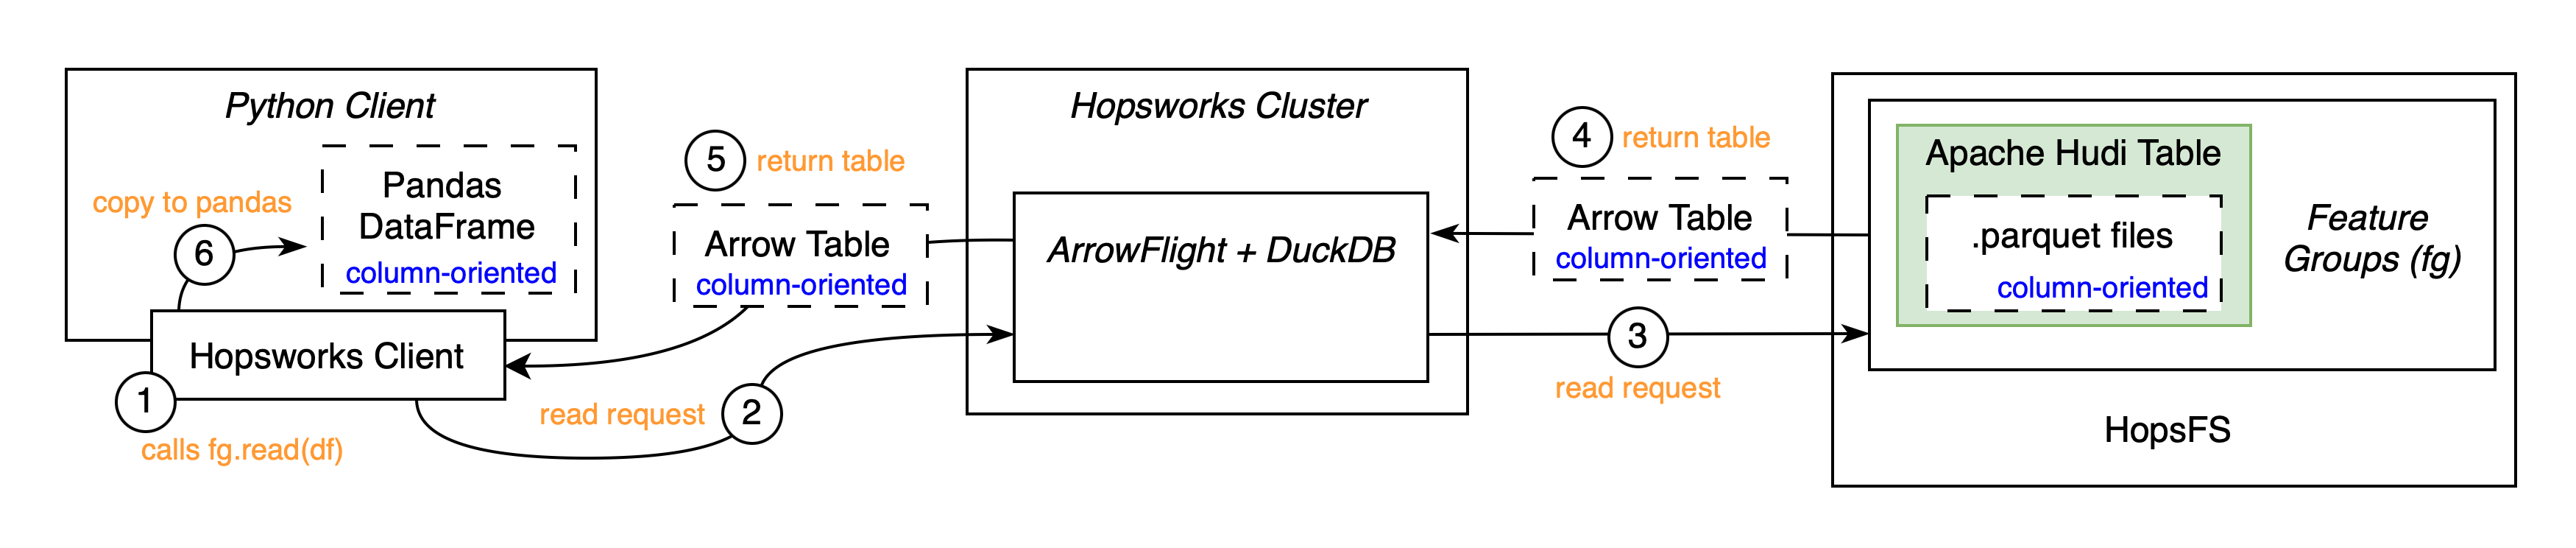
\includegraphics[width=\textwidth]{figures/2-background/FeatureStore-reading.png}
    \end{center}
    \caption{Legacy system reading process}
    \label{fig:featurestore_reading}
\end{figure}

\subsection{New system - Writing}

Figure \ref{fig:delta_rs_writing} shows how the delta-rs library writes on a Delta Lake table instanced on top of \gls{HopsFS}. The delta-rs library streamlines the process, without having to pass from a server instance (Spark).

\begin{figure}
    \begin{center}
      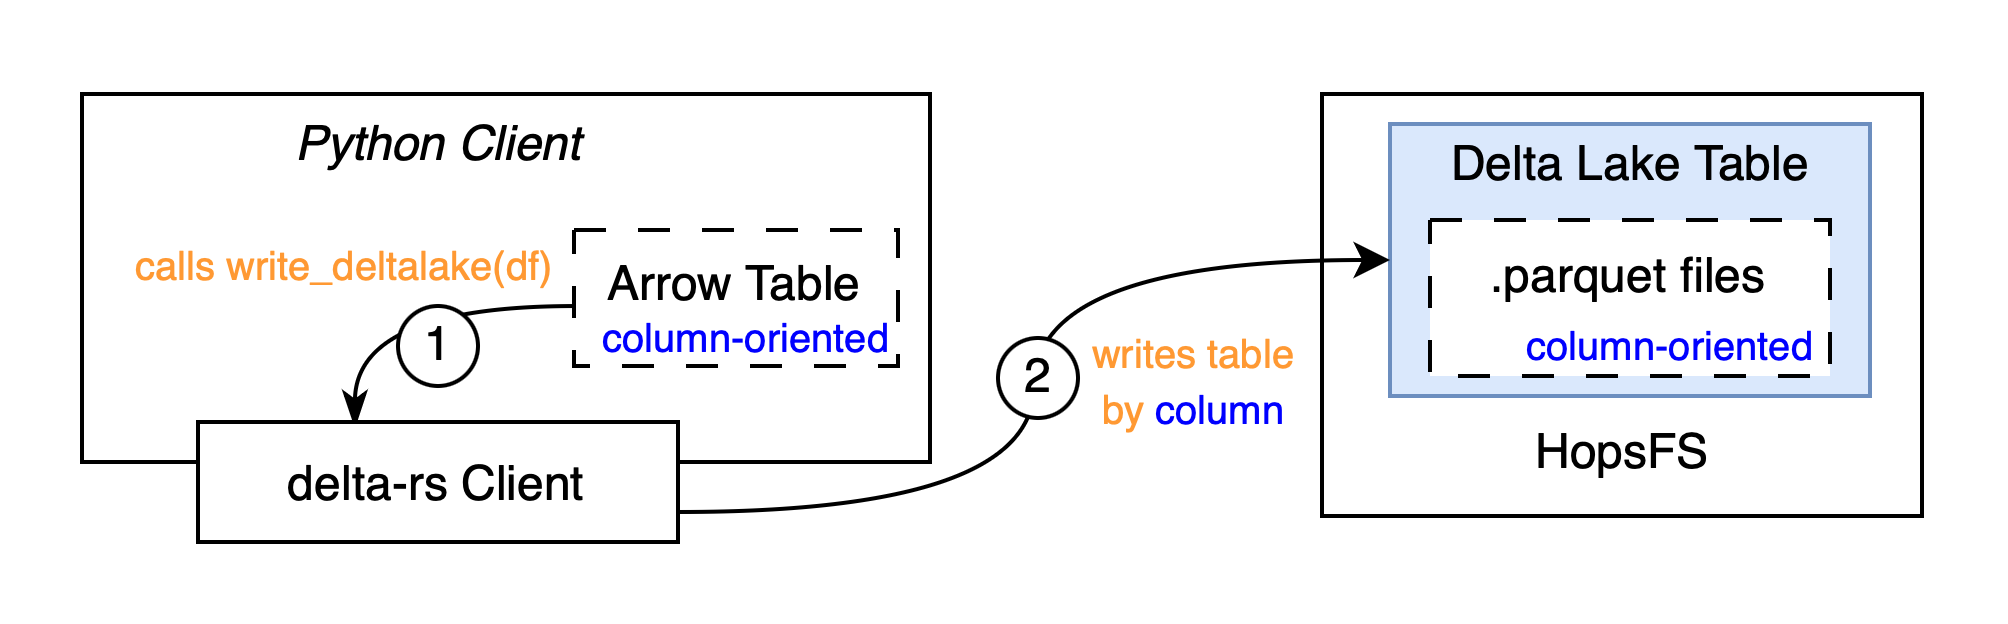
\includegraphics[width=\textwidth]{figures/2-background/delta-rs_writing.png}
    \end{center}
    \caption{delta-rs library writing process}
    \label{fig:delta_rs_writing}
\end{figure}

\subsection{New system - Reading}

Figure \ref{fig:delta_rs_reading} shows how the delta-rs library reads on a Delta Lake table instanced on top of \gls{HopsFS}. The delta-rs library streamlines the process, without having to pass from a server instance (Arrow Flight).

\begin{figure}
    \begin{center}
      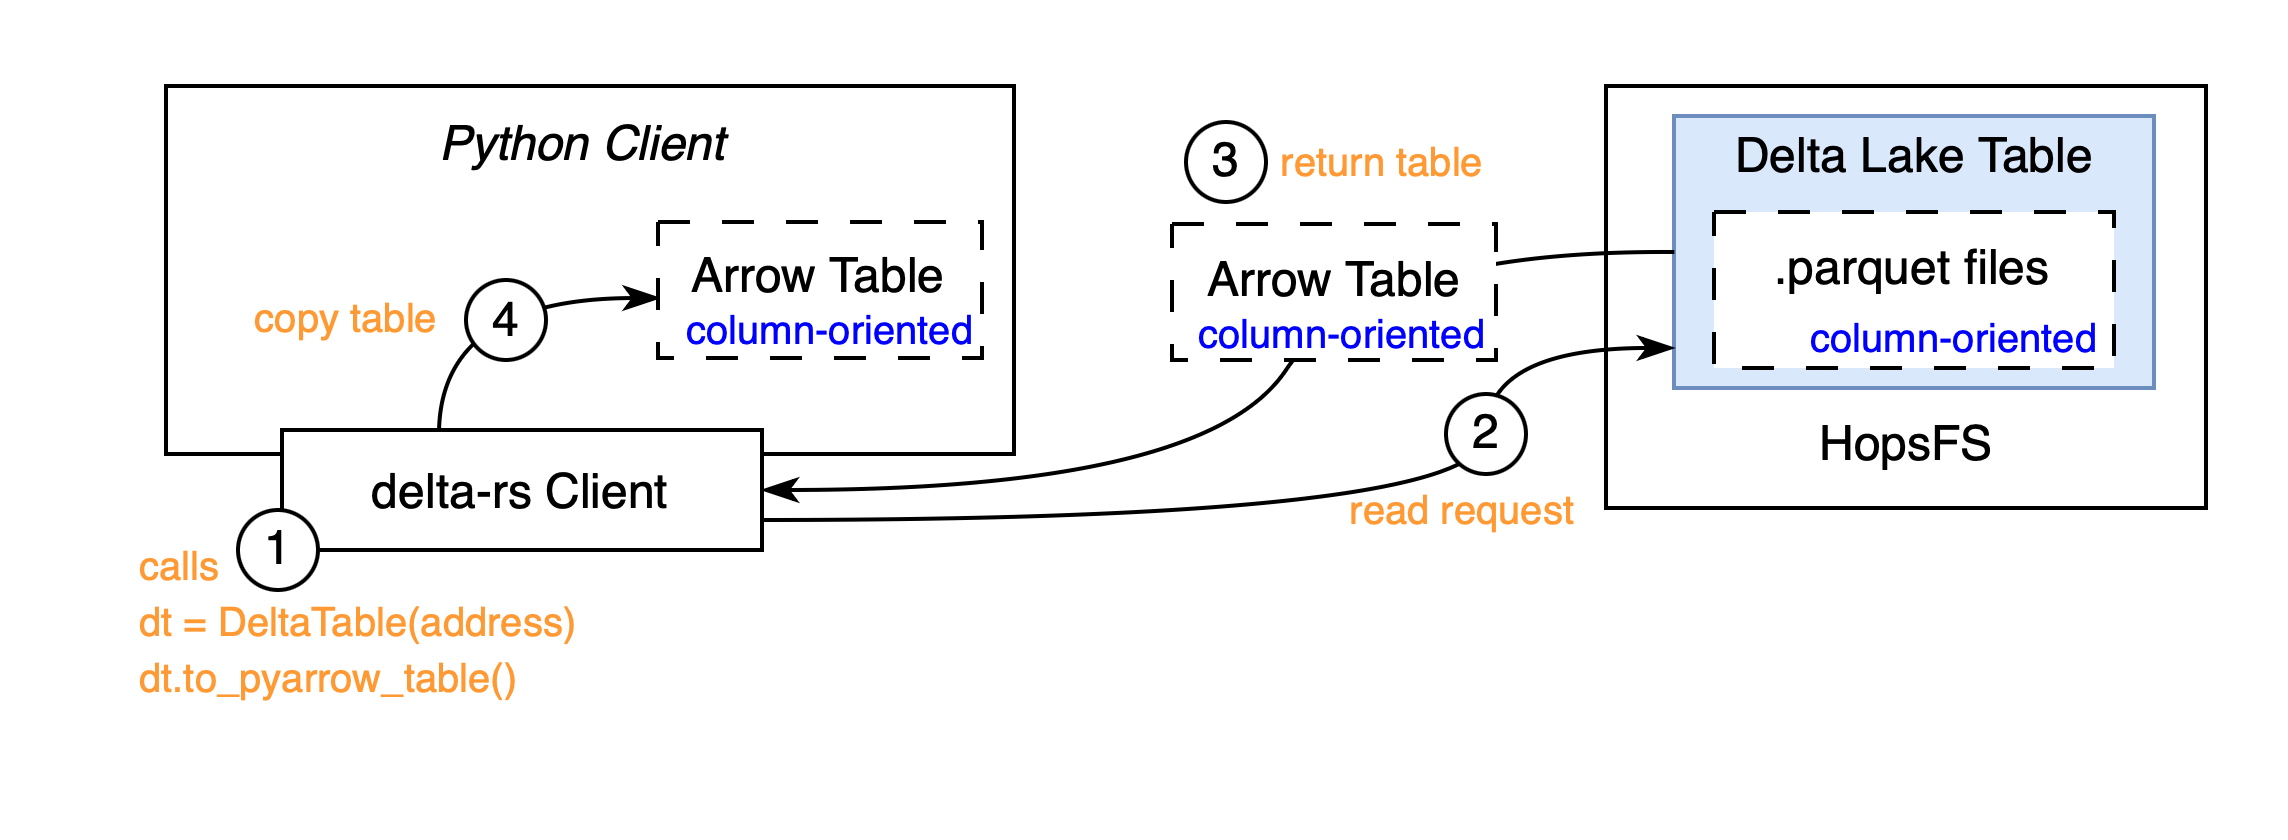
\includegraphics[width=\textwidth]{figures/2-background/delta-rs_reading.png}
    \end{center}
    \caption{delta-rs library reading process}
    \label{fig:delta_rs_reading}
\end{figure}